\documentclass[10pt]{article}

\usepackage{akteach}
\usepackage{amsmath}
\usepackage{amsfonts}
\usepackage{amssymb}
\usepackage{amsthm}
\usepackage{float}
\usepackage{algpseudocode}
\usepackage[all]{xy}


\newcommand{\C}{\mathbb{C}}
\newcommand{\Q}{\mathbb{Q}}
\newcommand{\K}{\mathbb{K}}
\newcommand{\proj}{\mathbb{P}}
\newcommand{\T}{\mathbb{T}}
\newcommand{\F}{\mathbb{F}}
\newcommand{\Z}{\mathbb{Z}}
\newcommand{\N}{\mathbb{N}}
\newcommand{\cp}{\mathbb{C}P}
\newcommand{\A}{\mathcal{A}}
\newcommand{\BB}{\mathcal{B}}
\newcommand{\CC}{\mathcal{C}}
\newcommand{\NN}{\mathcal{N}}
\newcommand{\MM}{\mathcal{M}}
\newcommand{\E}{\mathcal{E}}
\newcommand{\FF}{\mathcal{F}}
\newcommand{\G}{\mathcal{G}}
\newcommand{\eps}{\varepsilon}
\newcommand{\Hom}{\text{Hom}}
\newcommand{\Div}{\text{div}}
\newcommand{\Res}{\text{Res}}
\newcommand{\ord}{\text{ord}}
\newcommand{\Deg}{\text{deg}}
\newcommand{\mult}{\text{mult}}

\newcommand{\id}{\text{id}}
\newcommand{\Tr}{\text{Tr}}
\newcommand{\ad}{\text{ad}}
\newcommand{\Ad}{\text{Ad}}
\newcommand{\Aut}{\text{Aut}}
\newcommand{\der}{\text{der}}
\newcommand{\GL}{\text{GL}}
\newcommand{\gl}{\mathfrak{gl}}
\newcommand{\rad}{\mathfrak{rad}}
\newcommand{\inhook}{\hookrightarrow}
\newcommand{\sgn}{\text{sign}}

\begin{document}

\akteachheader{Numerical Analysis (CS 450)}%
{Homework Set 5, Bill Karr}

\akteachprobhead{%
  Problem 1: Interpolation, Newton and Cubic Splines (20 points)
}

\begin{itemize}

\item[(a)] (9 points) Prove that the formula using divided differences: \begin{align*}
f[t_1, t_2, ... ,t_k] &:= \frac{f[t_2, t_3, ... ,t_k] - f[t_1, t_2, ... ,t_{k-1}]}{t_k - t_1} \\
f[t_j] &:= f(t_j) \end{align*} indeed gives the coefficient of the $j$th basis function in the Newton interpolation polynomial.

\begin{proof}
Let $p_n$ denote the polynomial that interpolates $ f $ at $ t_1, ... , t_n $ for $ n = 1, 2, ... $. Let $ q $ denote the polynomial that interpolates $ f $ at $ t_2, ... , t_n $. Then, $$
p_n(x) = q(x) + \frac{x - t_n}{t_n - t_1}( q(x) - p_{n-1}(x) ).
$$ To see this, just evaluate both sides at $ t_k $. If $ k = n $, we obtain $$
f(t_n) = p(t_n) = q(t_n) + 0 = f(t_n).
$$  If $ k = 1 $, we obtain $ q(t_1) - ( q(t_1) - p_{n-1}(t_1) ) = p_{n-1}(t_1) = f(t_1) = p_n(t_n) $. Otherwise, $ q(t_k) = p_{n-1}(t_k) = f(t_k) $ and the equation holds at all $n$ points. Thus, the polynomials are equal on both sides.

The statement we want to prove is trivially true for degree zero polynomials. Suppose it holds for polynomials of degree $ 0, 1, ..., n-1 $. I played around with this for a while and I'm not sure where to go from here.
\end{proof}

\item[(b)] (6 points) Given the three data points $ (-1,1),(0,0),(1,1) $, determine the interpolating polynomial of degree two using the monomial, Lagrange, and Newton bases. Show that the three representations give the same polynomial.

\begin{proof}[Solution \& Proof]
For the monomial basis, we have $ m_0(t) = 1, m_1(t) = t, m_2(t) = t^2 $. Thus, we can set up the system of equations \begin{align*}
a \cdot 1 + b \cdot (-1) + c \cdot (-1)^2 = a - b + c &= 1 \\
a \cdot 1 + b \cdot (0) + c \cdot (0)^2 = a &= 0 \\
a \cdot 1 + b \cdot (1) + c \cdot (1)^2 = a + b + c &= 1 
\end{align*} to obtain $ a = 0, b = 0, c = 1 $. Thus, the interpolating polynomial in the monomial basis is $$
p(t) = 0 \cdot 1 + 0 \cdot t + 1 \cdot t^2 = t^2.
$$

For the Lagrange basis, we have \begin{align*}
\ell_0(t) &= \frac{(t - 0)(t - 1)}{(-1 - 0)(-1 - 1)} = \frac{t^2 - t}{2} \\
\ell_1(t) &= \frac{(t - (-1))(t - 1)}{(0 - (-1))(0 - 1)} = \frac{t^2 - 1}{-1} \\
\ell_2(t) &= \frac{(t - (-1))(t - 0)}{(1 - (-1))(1 - 0)} = \frac{t^2 + t}{2}
\end{align*} and the interpolating polynomial is given by $$
p(t) = 1 \cdot \ell_0(t) + 0 \cdot \ell_1(t) + 1 \cdot \ell_2(t)
= \frac{t^2 - t}{2} + \frac{t^2 + t}{2} = t^2.
$$

For the Newton basis, we have $ n_0(t) = 1, n_1(x) = t - (-1) = t+1, n_2(t) = (t+1)t = t^2 + t  $. We conclude the divided differences and obtain $$
y[-1] = y(-1) = 1, \quad y[-1,0] = \frac{0 - 1}{0 - (-1)} = -1, \quad y[-1,0,1] = \frac{y[1,0] - y[0,-1]}{1 - (-1)} = \frac{1 - (-1)}{2} = 1.
$$ Thus, Newton interpolation gives $$
p(t) = 1 \cdot 1 + (-1) \cdot (t+1) + 1 \cdot (t^2 + t) = t^2
$$

For each method, we obtain the same interpolating polynomial.
\end{proof}

\item[(c)]  (5 points) See \verb+splines.py+ for my code. Here is the plot I obtained. 

\begin{figure}[H]
  \centering
    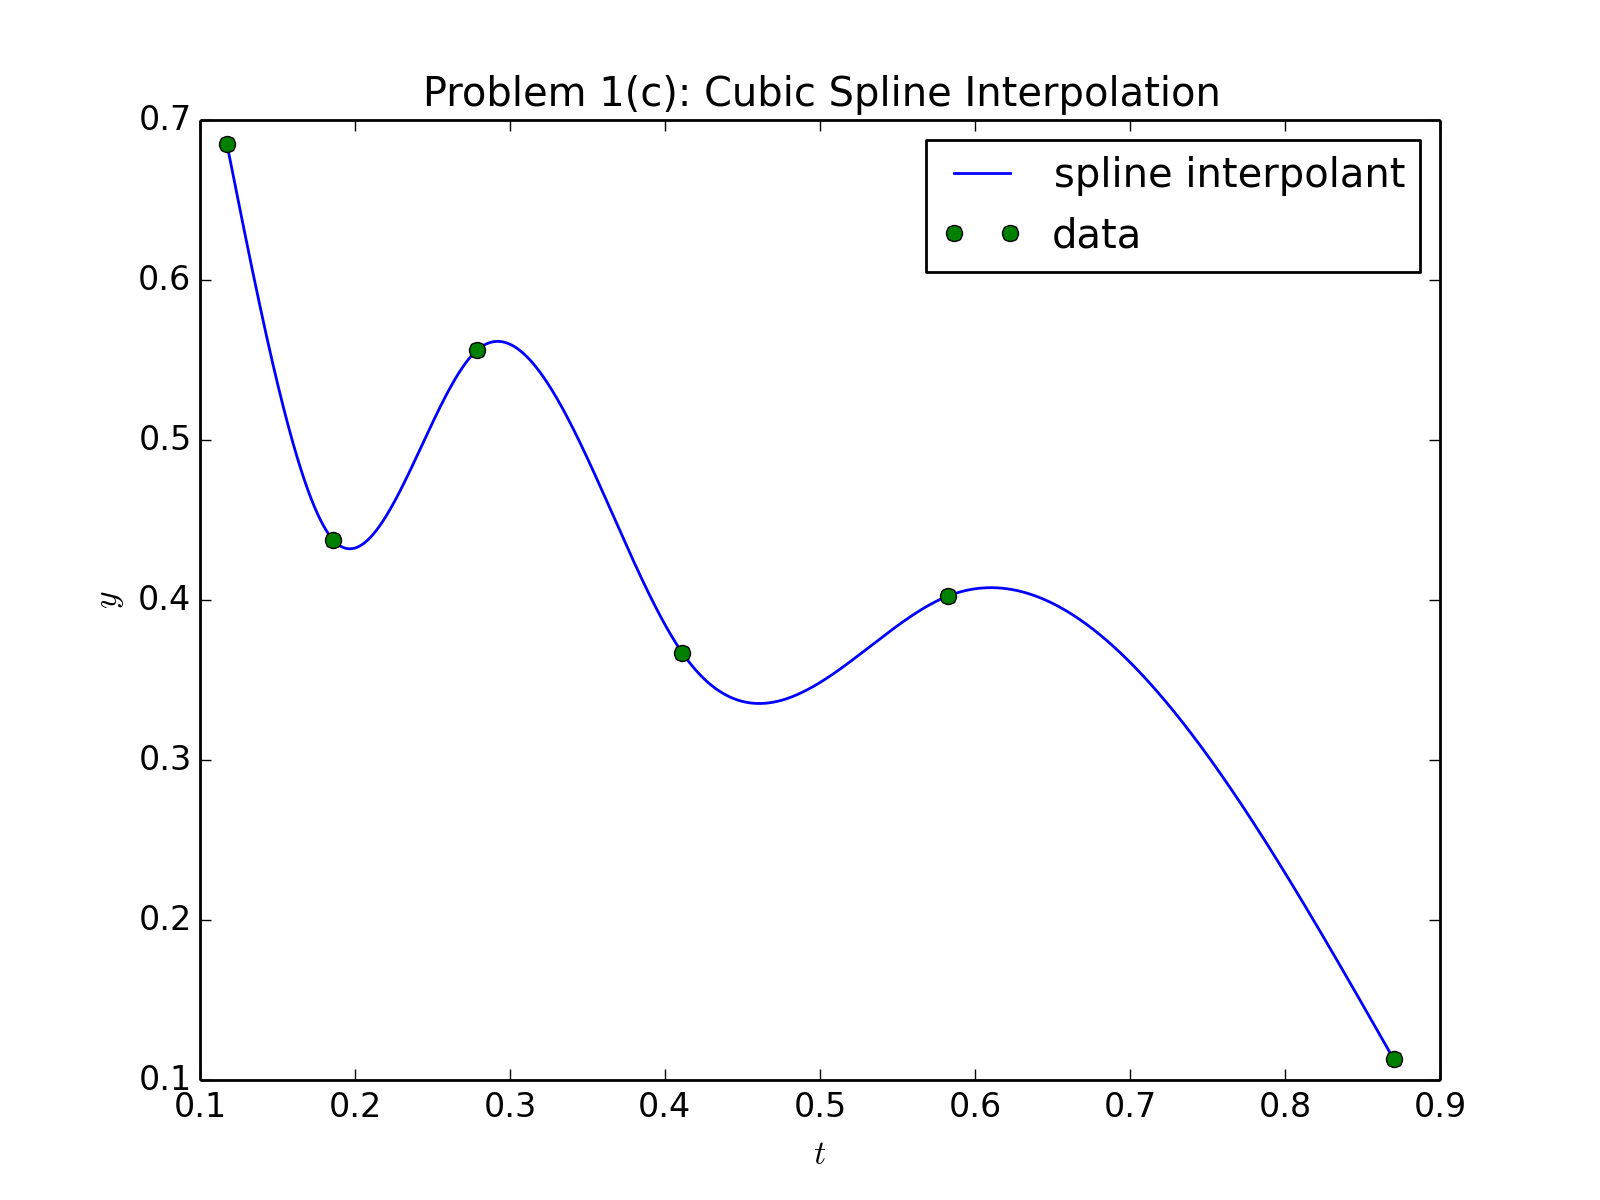
\includegraphics[scale=0.6]{spline}
\end{figure}

\end{itemize}

\akteachprobhead{%
  Problem 2: Numerical Quadrature (25 points)
}

See \verb+numerical_quad.py+ for my code.

\begin{itemize}
\item[(i)] My approximations were: \begin{verbatim}
For Midpoint rule:
Approximations of pi:
h = 2**-10, pi = 3.141592733218101, EOC = none
h = 2**-11, pi = 3.141592673477424, EOC = 2.00140996086
h = 2**-12, pi = 3.141592658559272, EOC = 2.00070491332
h = 2**-13, pi = 3.141592654831860, EOC = 2.00035226347
h = 2**-14, pi = 3.141592653900270, EOC = 2.00018416024
h = 2**-15, pi = 3.141592653667407, EOC = 2.00009079913
h = 2**-16, pi = 3.141592653609198, EOC = 1.9999339637
h = 2**-17, pi = 3.141592653594642, EOC = 2.0007596
h = 2**-18, pi = 3.141592653591006, EOC = 1.99920738298
h = 2**-19, pi = 3.141592653590098, EOC = 1.99314883259
h = 2**-20, pi = 3.141592653589872, EOC = 1.94633133521

For Trapezoid rule:
Approximations of pi:
h = 2**-10, pi = 3.141592494333178, EOC = none
h = 2**-11, pi = 3.141592613814530, EOC = 2.00140992462
h = 2**-12, pi = 3.141592643650833, EOC = 2.00070468768
h = 2**-13, pi = 3.141592651105661, EOC = 2.00035277923
h = 2**-14, pi = 3.141592652968836, EOC = 2.00017771168
h = 2**-15, pi = 3.141592653434568, EOC = 2.00012588161
h = 2**-16, pi = 3.141592653550985, EOC = 1.99993808964
h = 2**-17, pi = 3.141592653580094, EOC = 2.00046232817
h = 2**-18, pi = 3.141592653587369, EOC = 2.00026425406
h = 2**-19, pi = 3.141592653589195, EOC = 2.01995828714
h = 2**-20, pi = 3.141592653589640, EOC = 1.96819793991

For Simpson's rule:
Approximations of pi:
h = 2**-2, pi = 3.141591780936043, EOC = none
h = 2**-3, pi = 3.141592648320655, EOC = 7.37169855865
h = 2**-4, pi = 3.141592653535359, EOC = 6.59692064869
h = 2**-5, pi = 3.141592653589095, EOC = 6.2839905107
h = 2**-6, pi = 3.141592653589783, EOC = 6.15987133678

For Monte Carlo method:
Approximations of pi:
h = 2**-2, pi = 3.336361607500348, EOC = none
h = 2**-3, pi = 3.126671118885677, EOC = 3.70629589889
h = 2**-4, pi = 3.173248073913034, EOC = -1.08505662515
h = 2**-5, pi = 3.205488380443046, EOC = -1.01326689955
h = 2**-6, pi = 3.087227368889564, EOC = 0.233033748107
h = 2**-7, pi = 3.158107112667869, EOC = 1.71895598763
h = 2**-8, pi = 3.138802232736366, EOC = 2.56517508377
h = 2**-9, pi = 3.077842286669497, EOC = -4.51387901358
h = 2**-10, pi = 3.167965867109579, EOC = 1.27336027432
h = 2**-11, pi = 3.168738485529880, EOC = -0.041657327689
h = 2**-12, pi = 3.153660735662613, EOC = 1.16953428578
h = 2**-13, pi = 3.131703274208692, EOC = 0.287244522115
h = 2**-14, pi = 3.137751019590208, EOC = 1.3641599089
h = 2**-15, pi = 3.146065699961296, EOC = -0.219537637645
h = 2**-16, pi = 3.141329062869102, EOC = 4.08488622618
h = 2**-17, pi = 3.139000109511650, EOC = -3.29799702931
h = 2**-18, pi = 3.143423662383446, EOC = 0.501729797907
h = 2**-19, pi = 3.142512928700046, EOC = 0.992501604829
h = 2**-20, pi = 3.141344166315301, EOC = 1.88889323942
h = 2**-21, pi = 3.141500851323004, EOC = 1.43657028818
\end{verbatim}

\item[(ii)] See above for my empirical order of convergence values. Here is my plot of the relative errors with best fit curves for the four methods:

\begin{figure}[H]
  \centering
    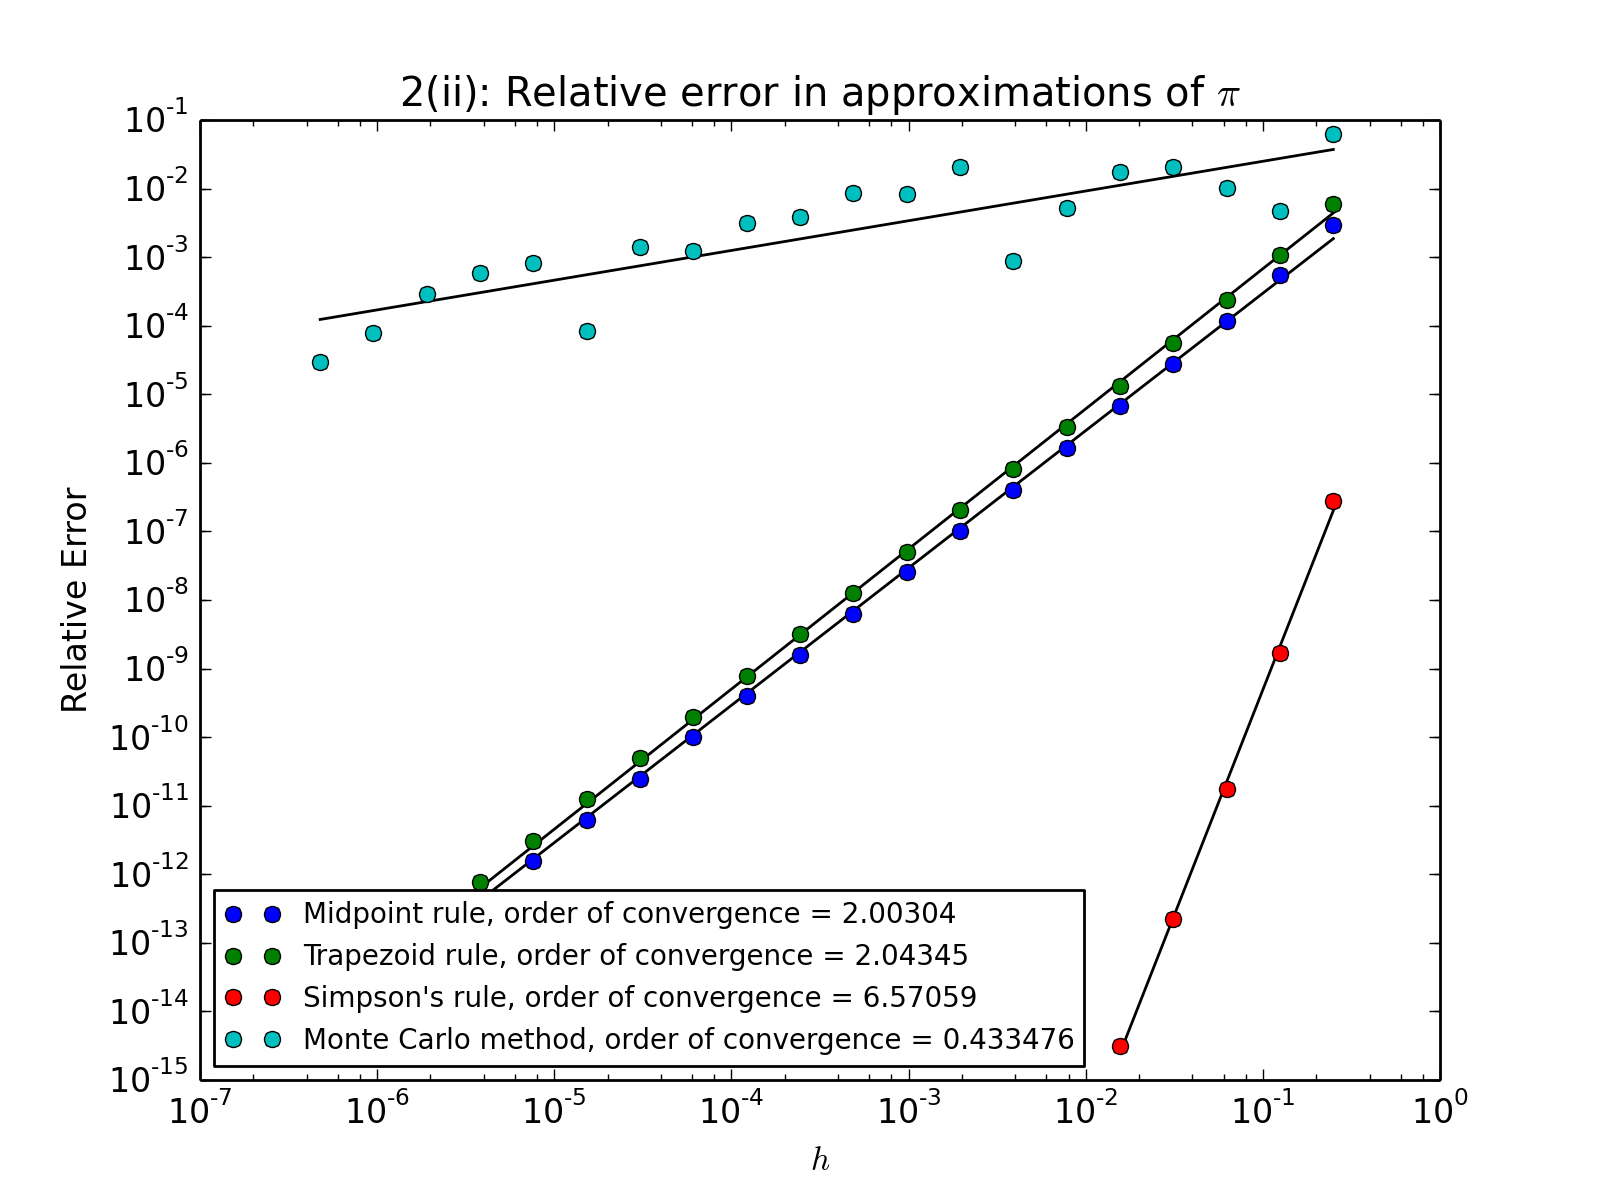
\includegraphics[scale=0.6]{pi}
\end{figure}

\item[(iii)] When I push my code to the limit with $ h \approx 0 $, the results stop improving in accuracy once the relative error gets close to machine precision. Below is a graph showing this. I omitted the legend, but the color coding is the same as above.

\begin{figure}[H]
  \centering
    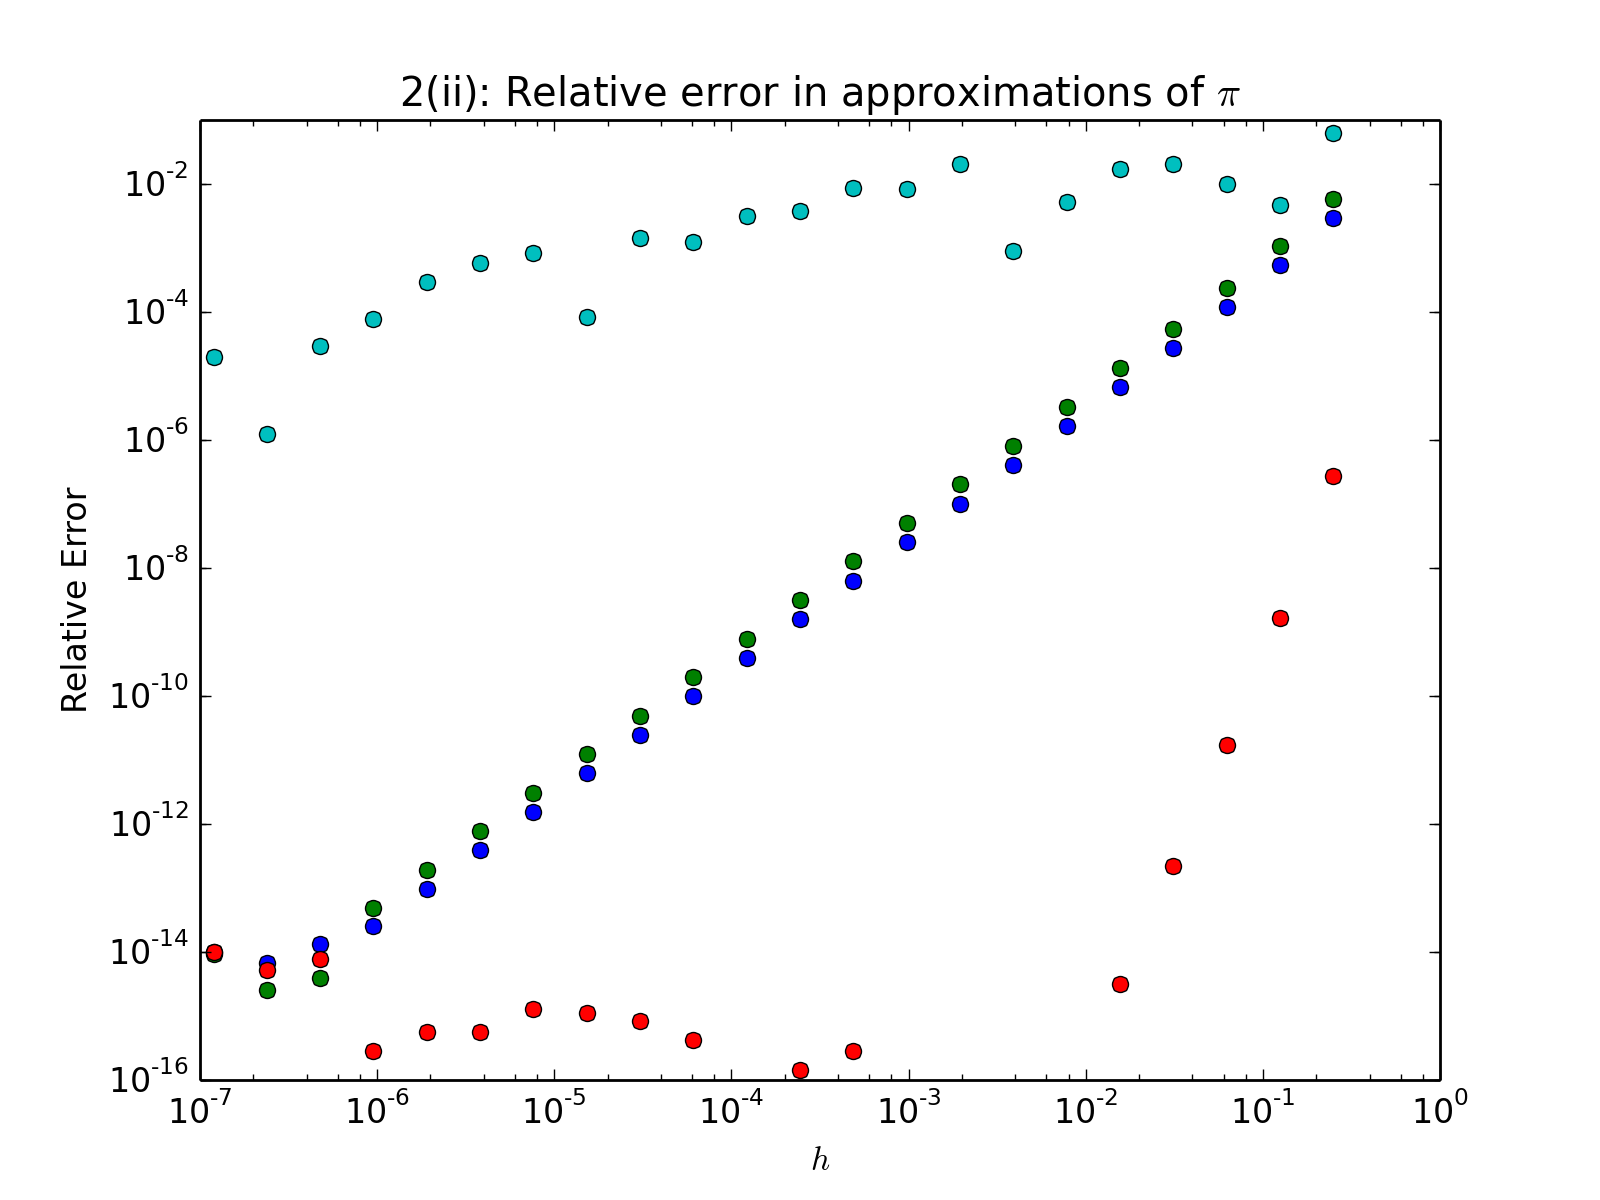
\includegraphics[scale=0.6]{pi_limits}
\end{figure}

\end{itemize}

\newpage

\akteachprobhead{%
  Problem 3: Gaussian Quadrature (20 points)
}

\begin{itemize}

\item[(a)] Let $p$ be a real polynomial of degree $n$ such that: $$
\int_{a}^b p(x) x^k \, dx = 0, \quad k = 0, 1, ..., n-1.
$$ \begin{itemize}
\item[(i)] Show that the $n$ zeros of $p$ are real, simple, and lie on the open interval $ (a,b) $.

\begin{proof}
First, note that any root of $p(x)$ of odd order must be real.
Let $ q(x) = (x - x_1) \cdots (x - x_k) $ where $ x_1, ... , x_k $ the distinct real odd-order roots of $ p(x) $ (note: $ k \leq n $). Then, $ p(x)q(x) $ does not change sign on $ [a,b] $. Thus, $ \int_{a}^b p(x)q(x) \, dx \neq 0 $ and $ \deg(q(x)) = k \geq n \Rightarrow k = n $. Since $p(x)$ has degree $n$ and $ x_1, ... , x_n $ are real roots, it must be that they are all of the roots of $p$ and must be simple.
\end{proof}

\item[(ii)] Show that the $n$-point interpolatory quadrature on $ [a,b] $ whose nodes are the zeros of $p$ has degree $2n-1$.

\begin{proof}
Denote $ Q(f) = \sum_{k=1}^n w_k f(x_k) $ as the interpolatory quadrature of a function $f$ using the roots of $p$ as nodes where $ w_j $ are the weights.

Consider a polynomial $ f(x) $ of degree $ \leq 2n - 1 $. Perform polynomial long division to obtain $ f(x) = p(x)q(x) + r(x) $ where $ p,r $ have degree $ \leq n-1 $. We know interpolatory quadrature is exact for polynomials $ < n $ since we have $n$ nodes. Using the fact that $p$ is orthogonal to $q$ (by definition, $p$ is orthogonal to any polynomial of degree $ < n $), $$
\int_a^b f(x) \, dx = \int_a^b p(x)q(x) + r(x) \, dx = \int_a^b p(x)q(x) \, dx + \int_a^b r(x) \, dx = \int_a^b r(x) \, dx = Q(r). $$

However, since $ p(x_k) = 0 $, $$
Q(f) = \sum_{k = 1}^n w_k ( p(x_k)q(x_k) + r(x_k) ) = \sum_{k = 1}^n w_k  r(x_k) = Q(r) = \int_a^b f(x) \, dx.
$$ Thus, $ Q $ is exact for $f$, i.e. any polynomial of degree $ \leq 2n-1 $.
\end{proof}
\end{itemize}

\item[(b)] See \verb+guassian_quad.py+ for my code.

\item[(c)] The first function does not obey $ E(h) \approx Ch^p $, but the expected error does get small quickly as $ h \to 0 $. The latter obeys $ E(h) \approx C h^2 $, although it changes $C$ value depending on whether $n = 1/h$ is odd or even. This is because the Gauss-Legendre nodes are distributed in different ways for even and odd numbers.

Here are the plots of the errors for various $h$ values of the two functions.

\begin{figure}[H]
  \centering
    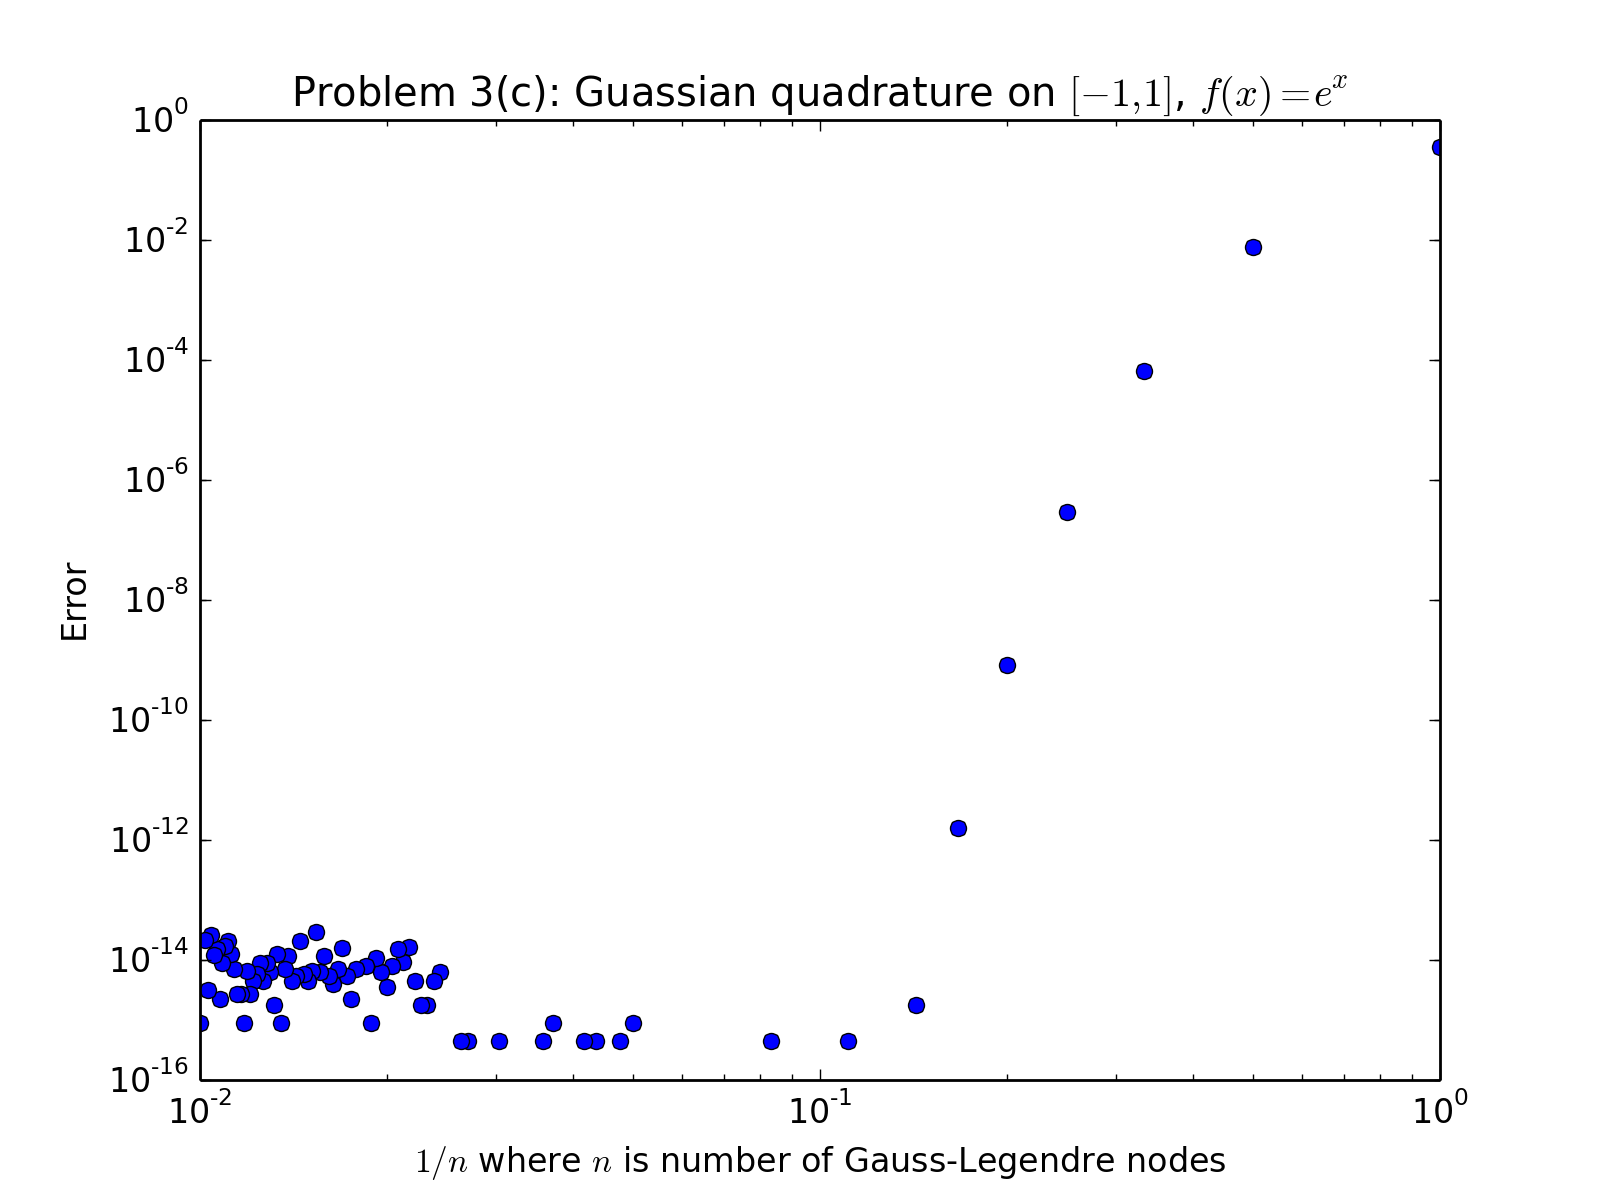
\includegraphics[scale=0.6]{gauss0}
\end{figure}

\begin{figure}[H]
  \centering
    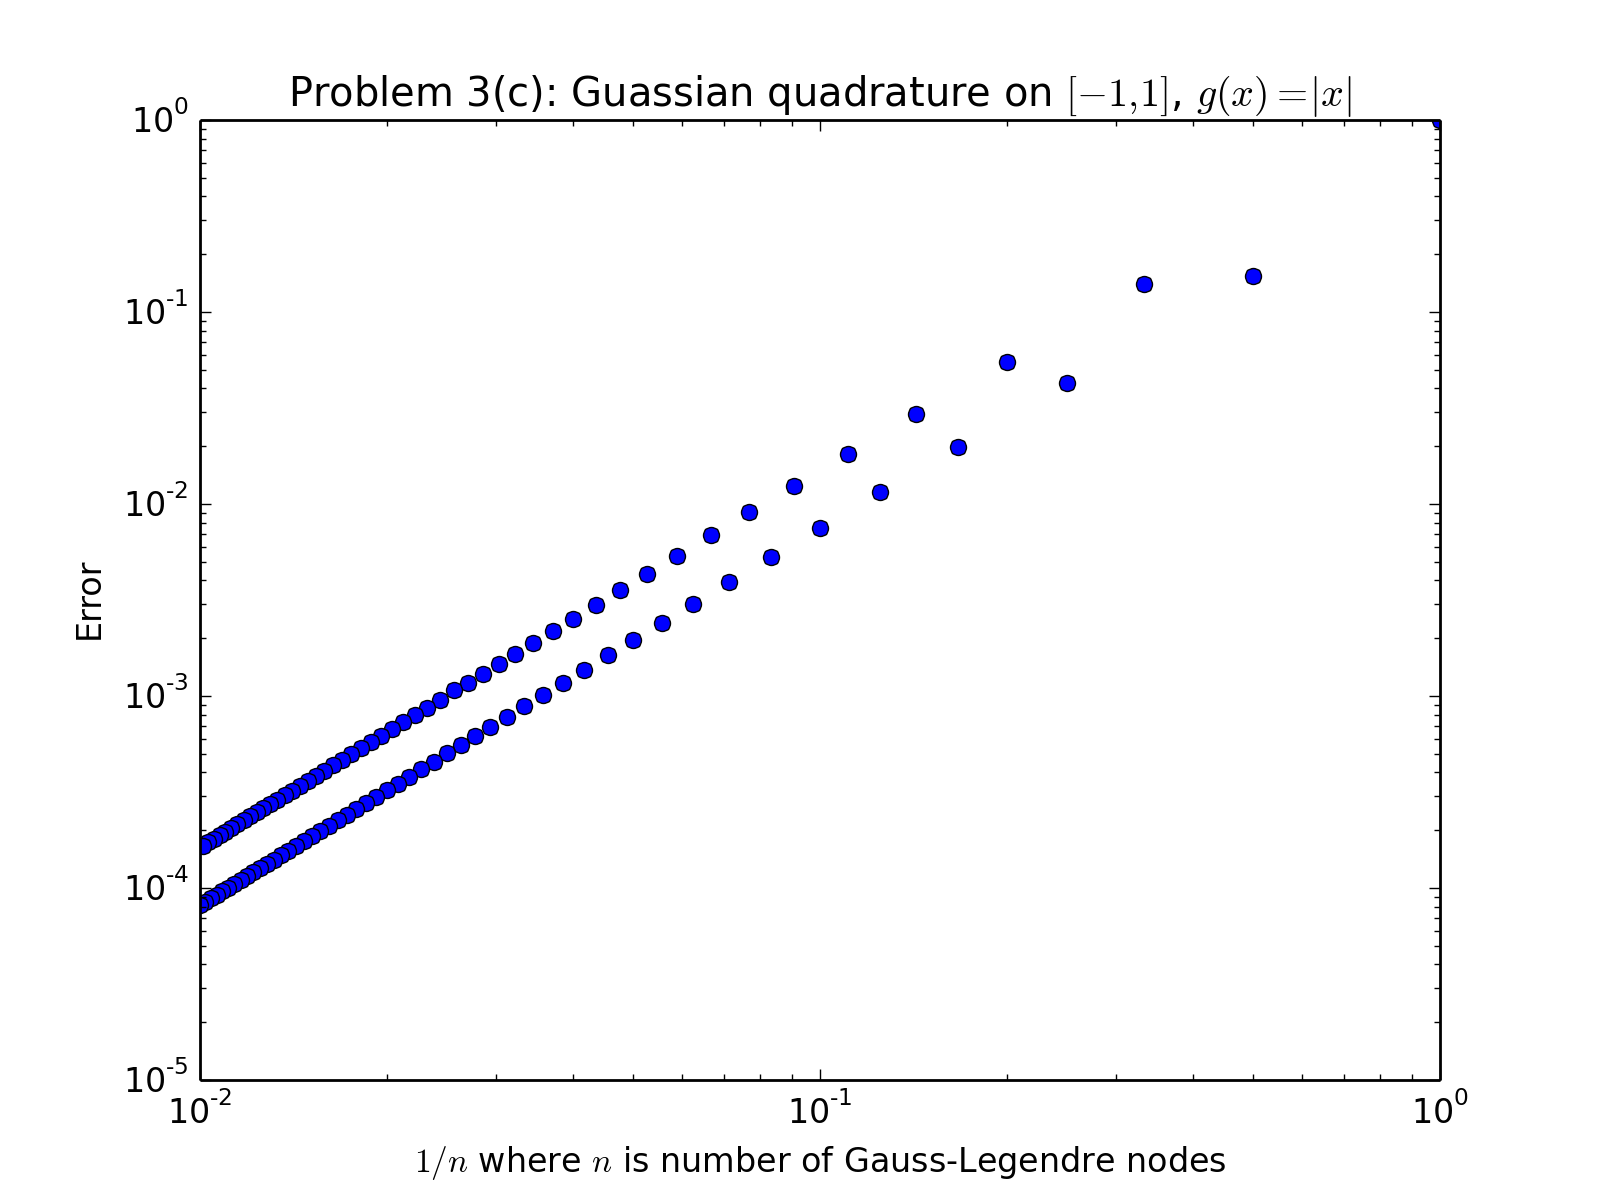
\includegraphics[scale=0.6]{gauss1}
\end{figure}
\end{itemize}

\newpage

\akteachprobhead{%
  Problem 4: Numerical Differentiation (15 points)
}

\begin{itemize}

\item[(a)] Note that $$
f(x+h) = f(x) + hf'(x) + \frac{h^2}{2} f''(x) + O(h^3)
$$  and thus, $$
f(x+ 2h) = f(x) + 2hf'(x) + 2 h^2 f''(x) + O(h^3).
$$ In order to get the $f(x)$ and $ f''(x) $ terms to cancel, we can take $ -3 f(x) + 4f(x+h) - f(x+2h) $ and obtain $$
-3 f(x) + 4f(x+h) - f(x+2h) = 2h f'(x) + O(h^3).
$$ Solving for $ f'(x) $, we obtain $$
f'(x) = \frac{-3 f(x) + 4f(x+h) - f(x+2h)}{2h} + O(h^2).
$$

\item[(b)] See \verb+differentiation.py+ for my code.

\item[(c)] The expected order of convergence is 2 by the above formula. I observe a convergence rate of 2 until $ h \approx 10^{-5} $. Then the error starts increasing. This is likely due to errors in the way \verb+numpy+ computes $\cos(x)$ and $ \sin(x) $ as well as computational errors.  Here is my plot:

\begin{figure}[H]
  \centering
    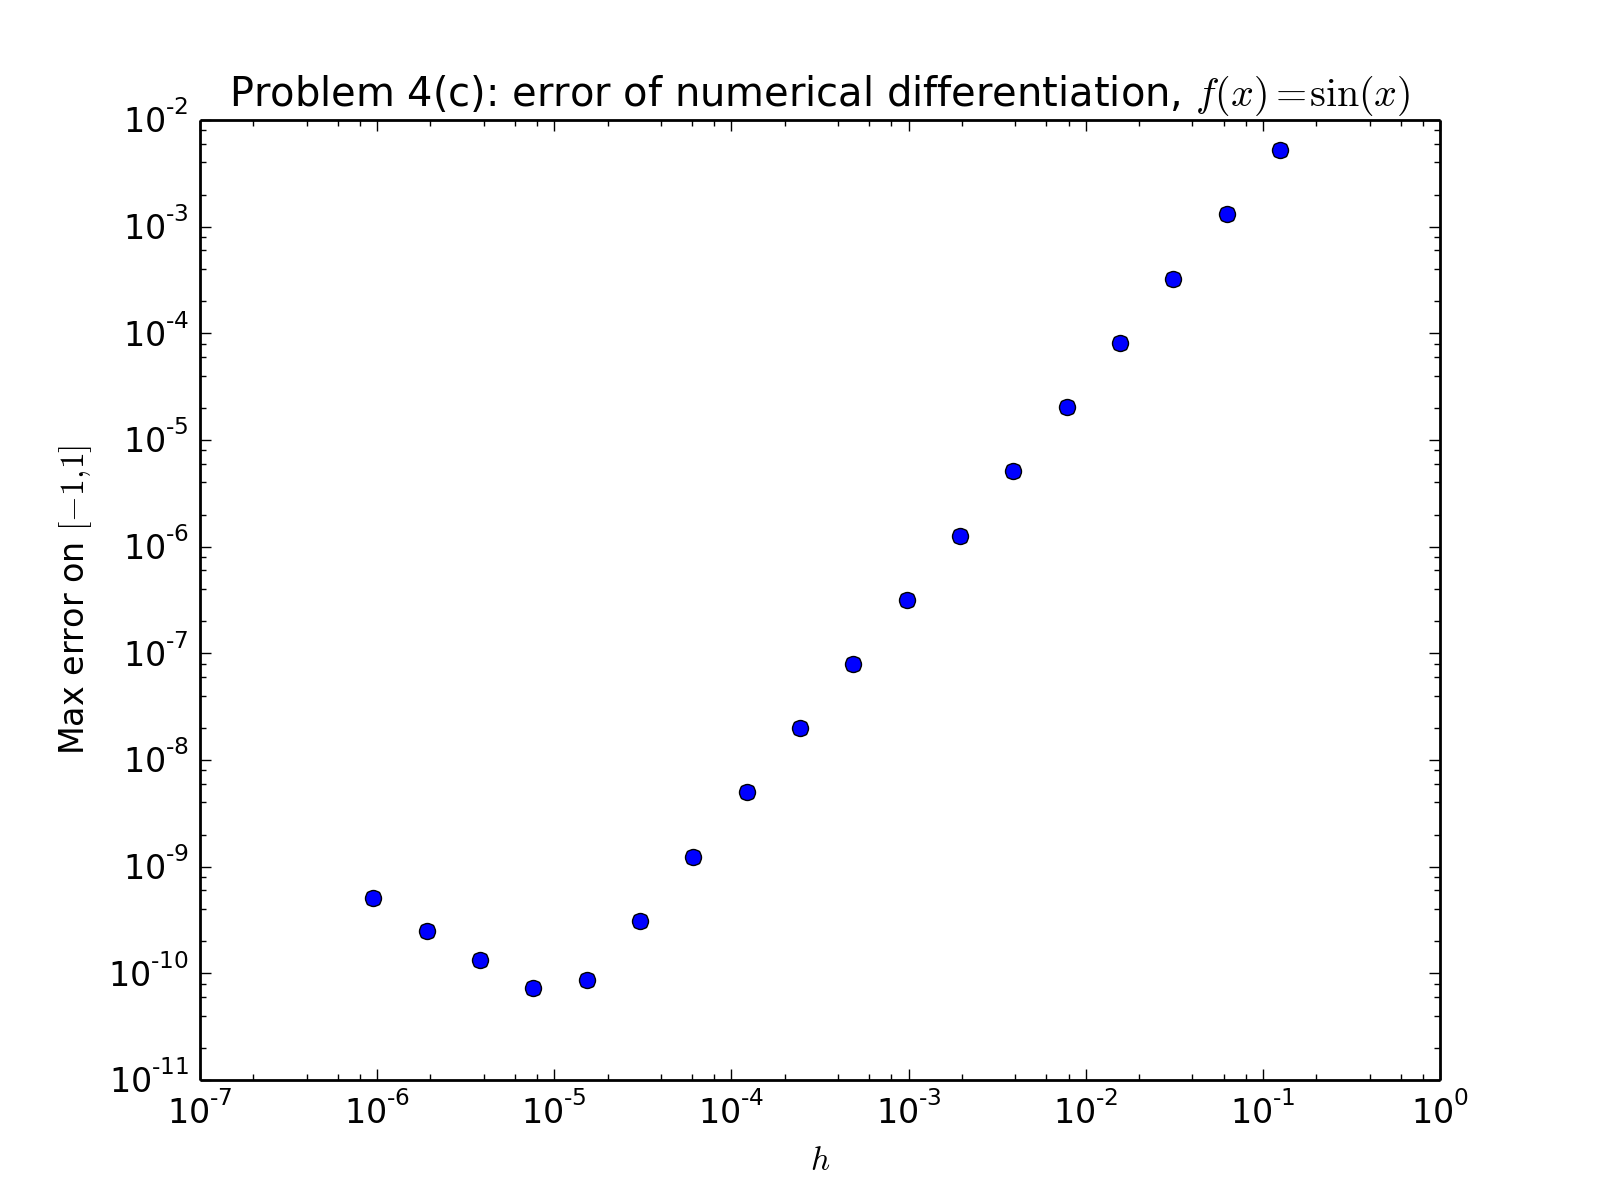
\includegraphics[scale=0.6]{diff}
\end{figure}

\end{itemize}

\newpage

\akteachprobhead{%
  Problem 5: Initial Value Problems (20 points)
}

See \verb+ivps.py+ for my code.

\begin{itemize}

\item[(a)] For Forward Euler method,  Here are my plots.

\begin{figure}[H]
  \centering
    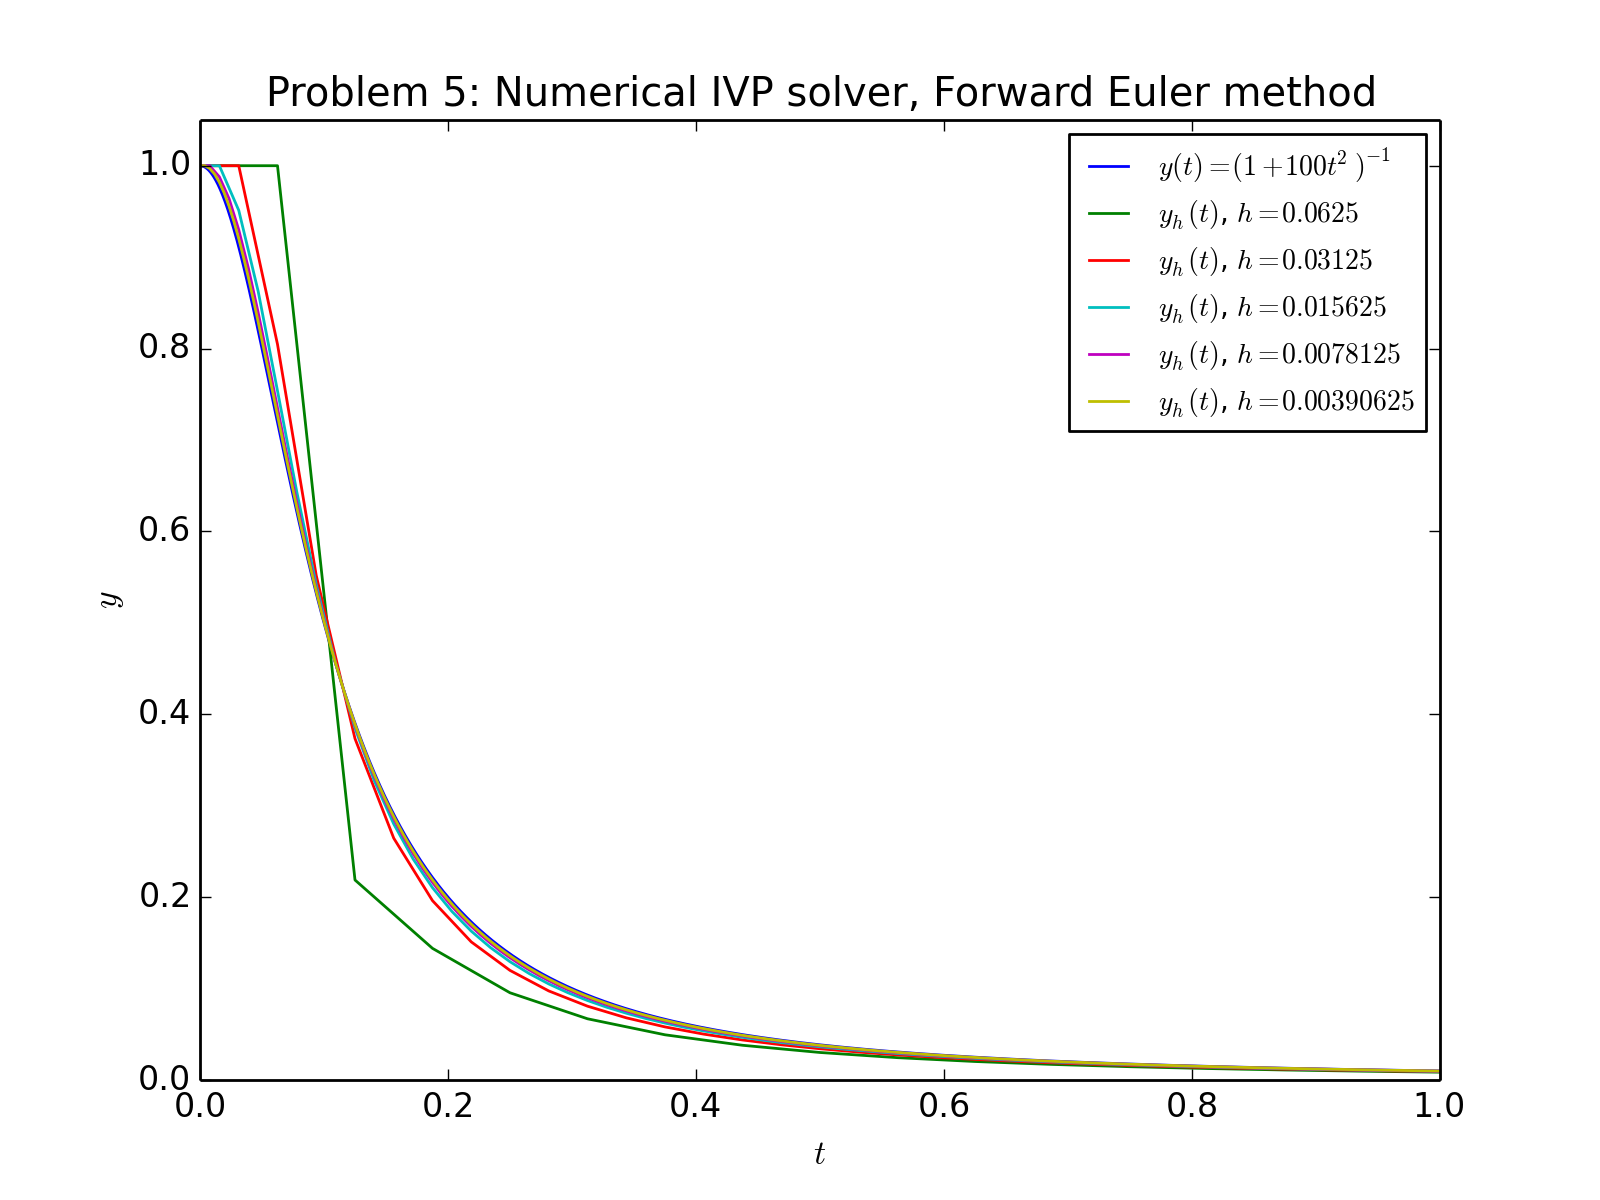
\includegraphics[scale=0.6]{ivp_sol_f}
\end{figure}

\begin{figure}[H]
  \centering
    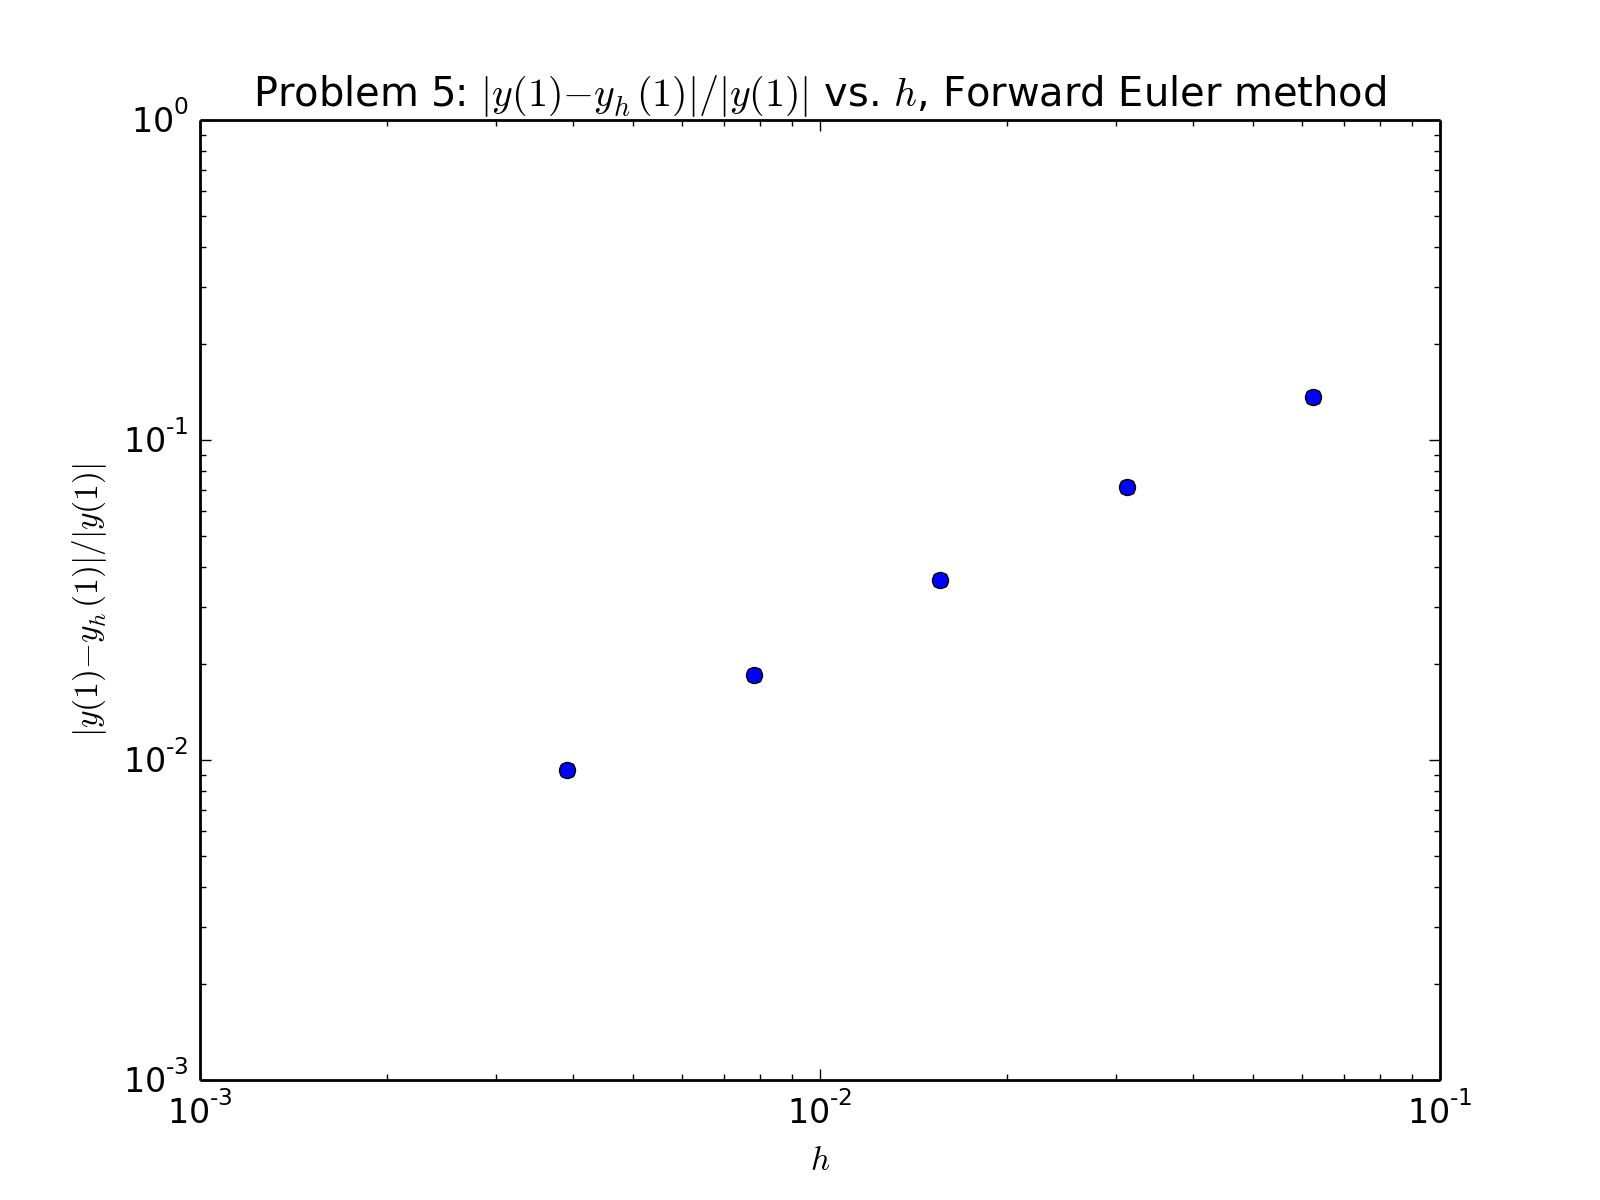
\includegraphics[scale=0.6]{ivp_err_f}
\end{figure}

E.O.C. values: 0.93459598,  0.96506194,  0.98311564,  0.99166013.

Looks stable! As $h \to 0$, the approximate solutions are close to the true solution.

\newpage

\item[(b)] For Backward Euler method, here are my plots.

\begin{figure}[H]
  \centering
    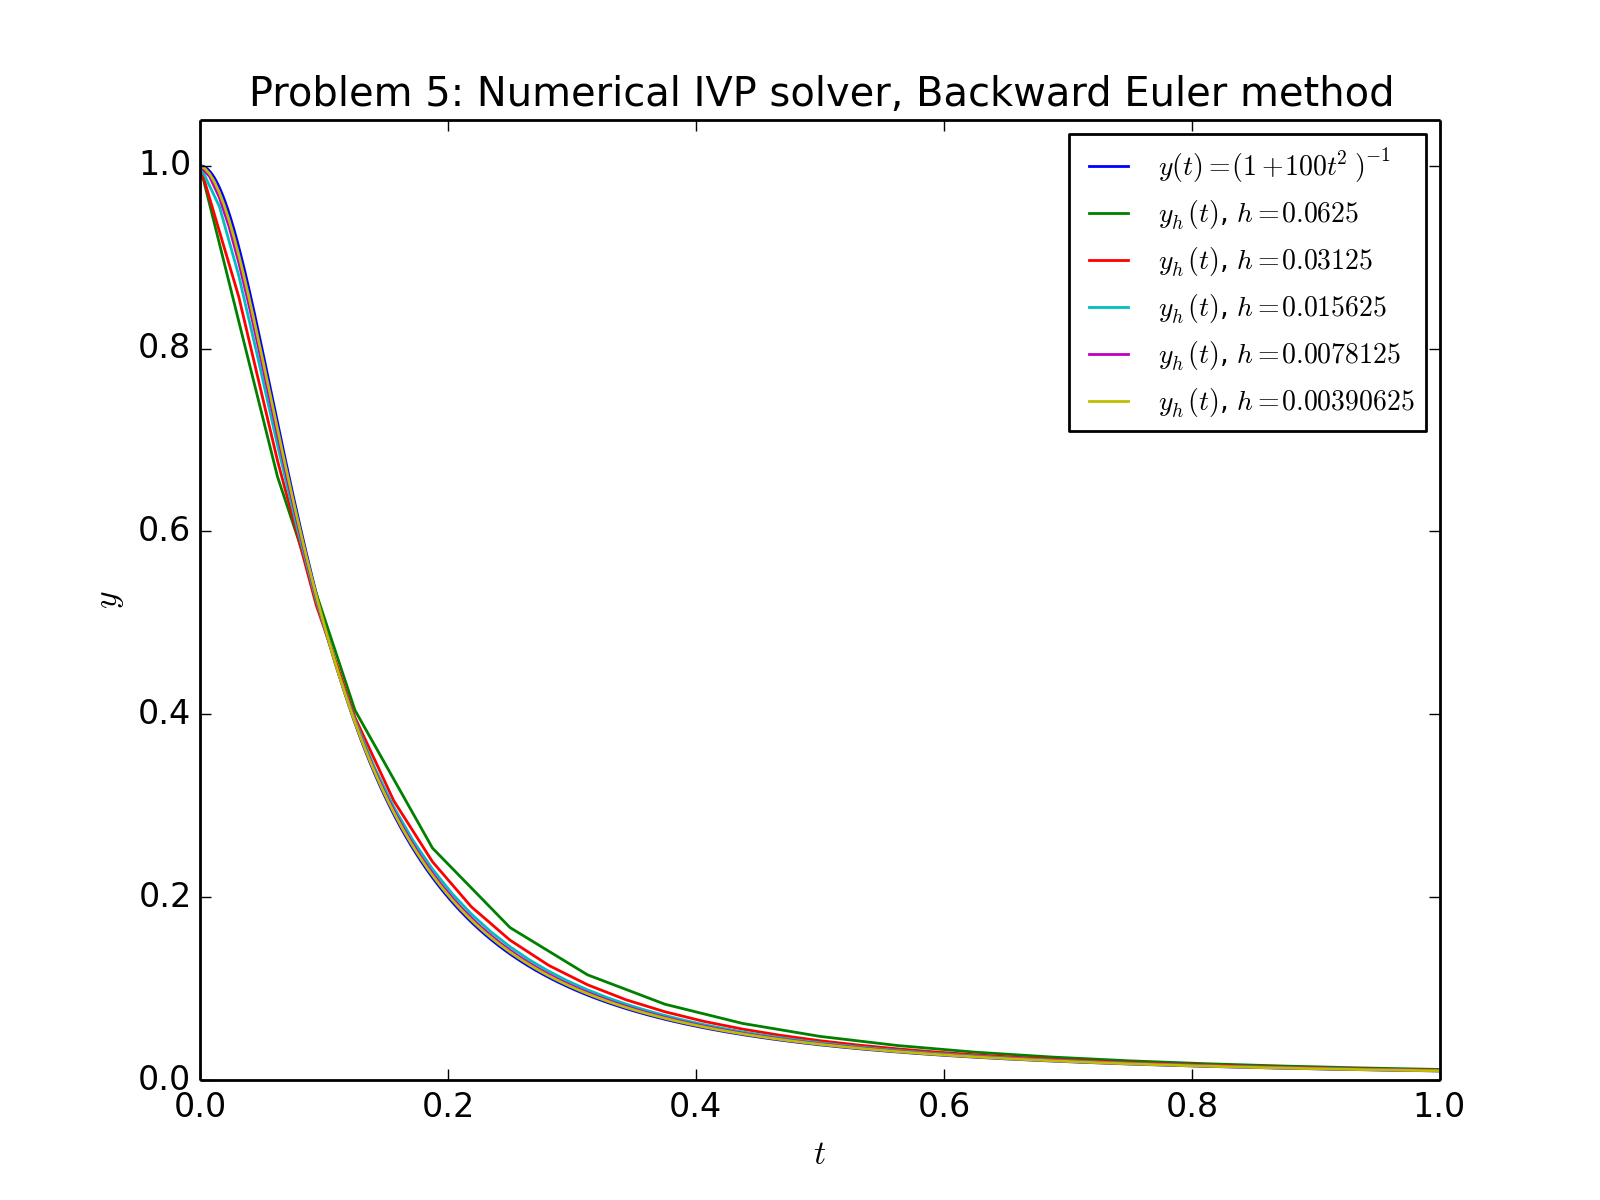
\includegraphics[scale=0.6]{ivp_sol_b}
\end{figure}

\begin{figure}[H]
  \centering
    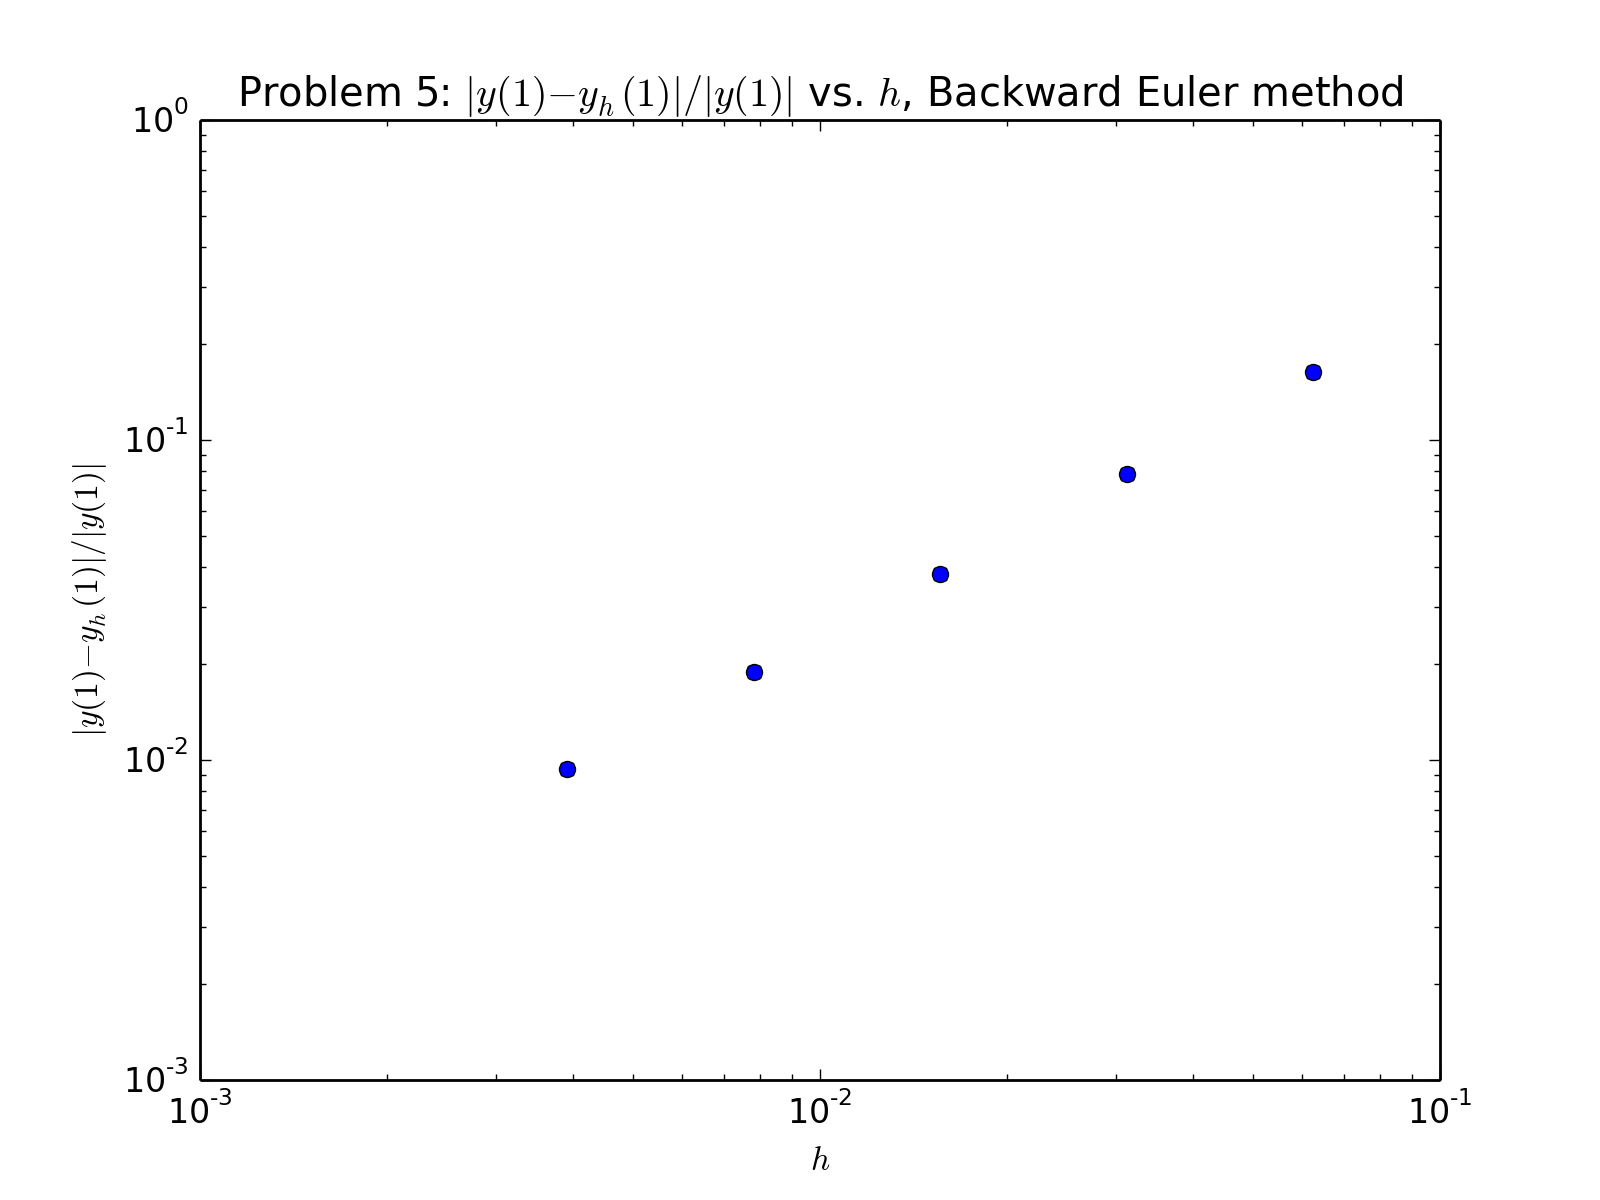
\includegraphics[scale=0.6]{ivp_err_b}
\end{figure}

E.O.C. values: 1.06632339,  1.0327388,   1.01636717,  1.0082122.

Looks stable! As $h \to 0$, the approximate solutions are close to the true solution.

\newpage

\item[(c)] For Fourth-order Runge-Kutta method, here are my plots.

\begin{figure}[H]
  \centering
    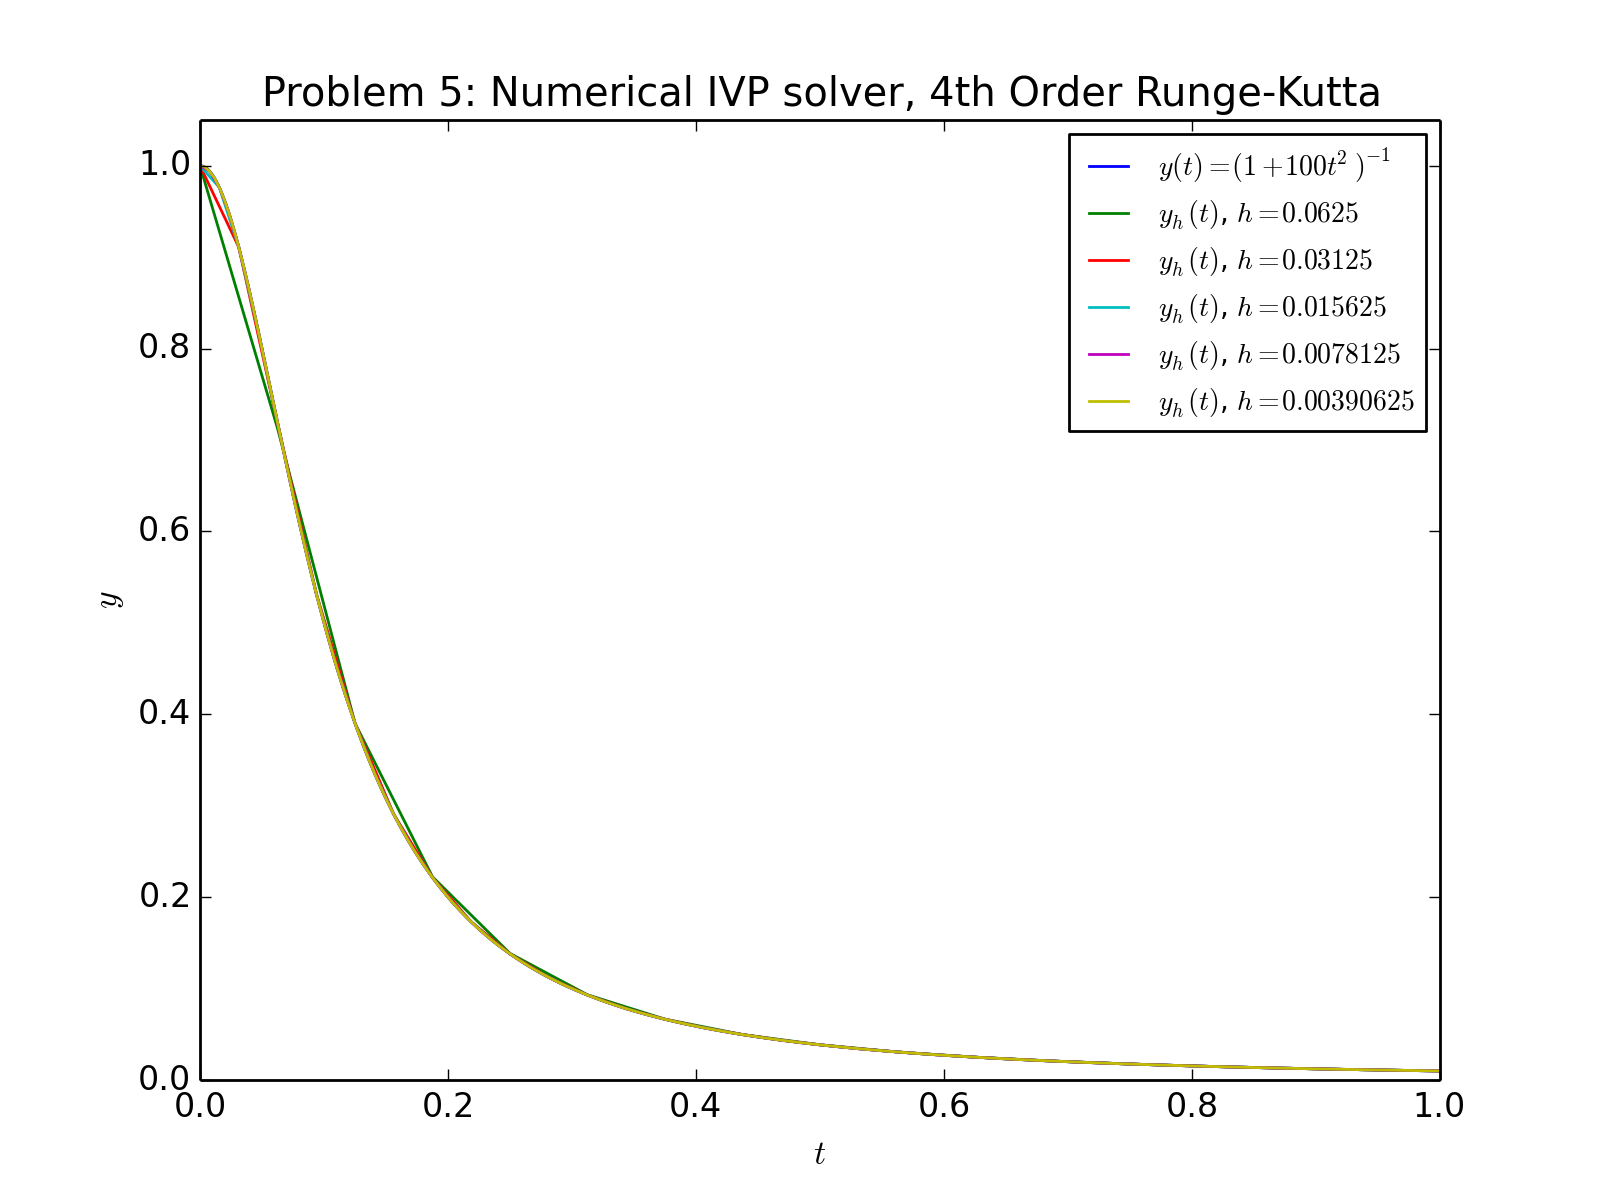
\includegraphics[scale=0.6]{ivp_sol_rk}
\end{figure}

\begin{figure}[H]
  \centering
    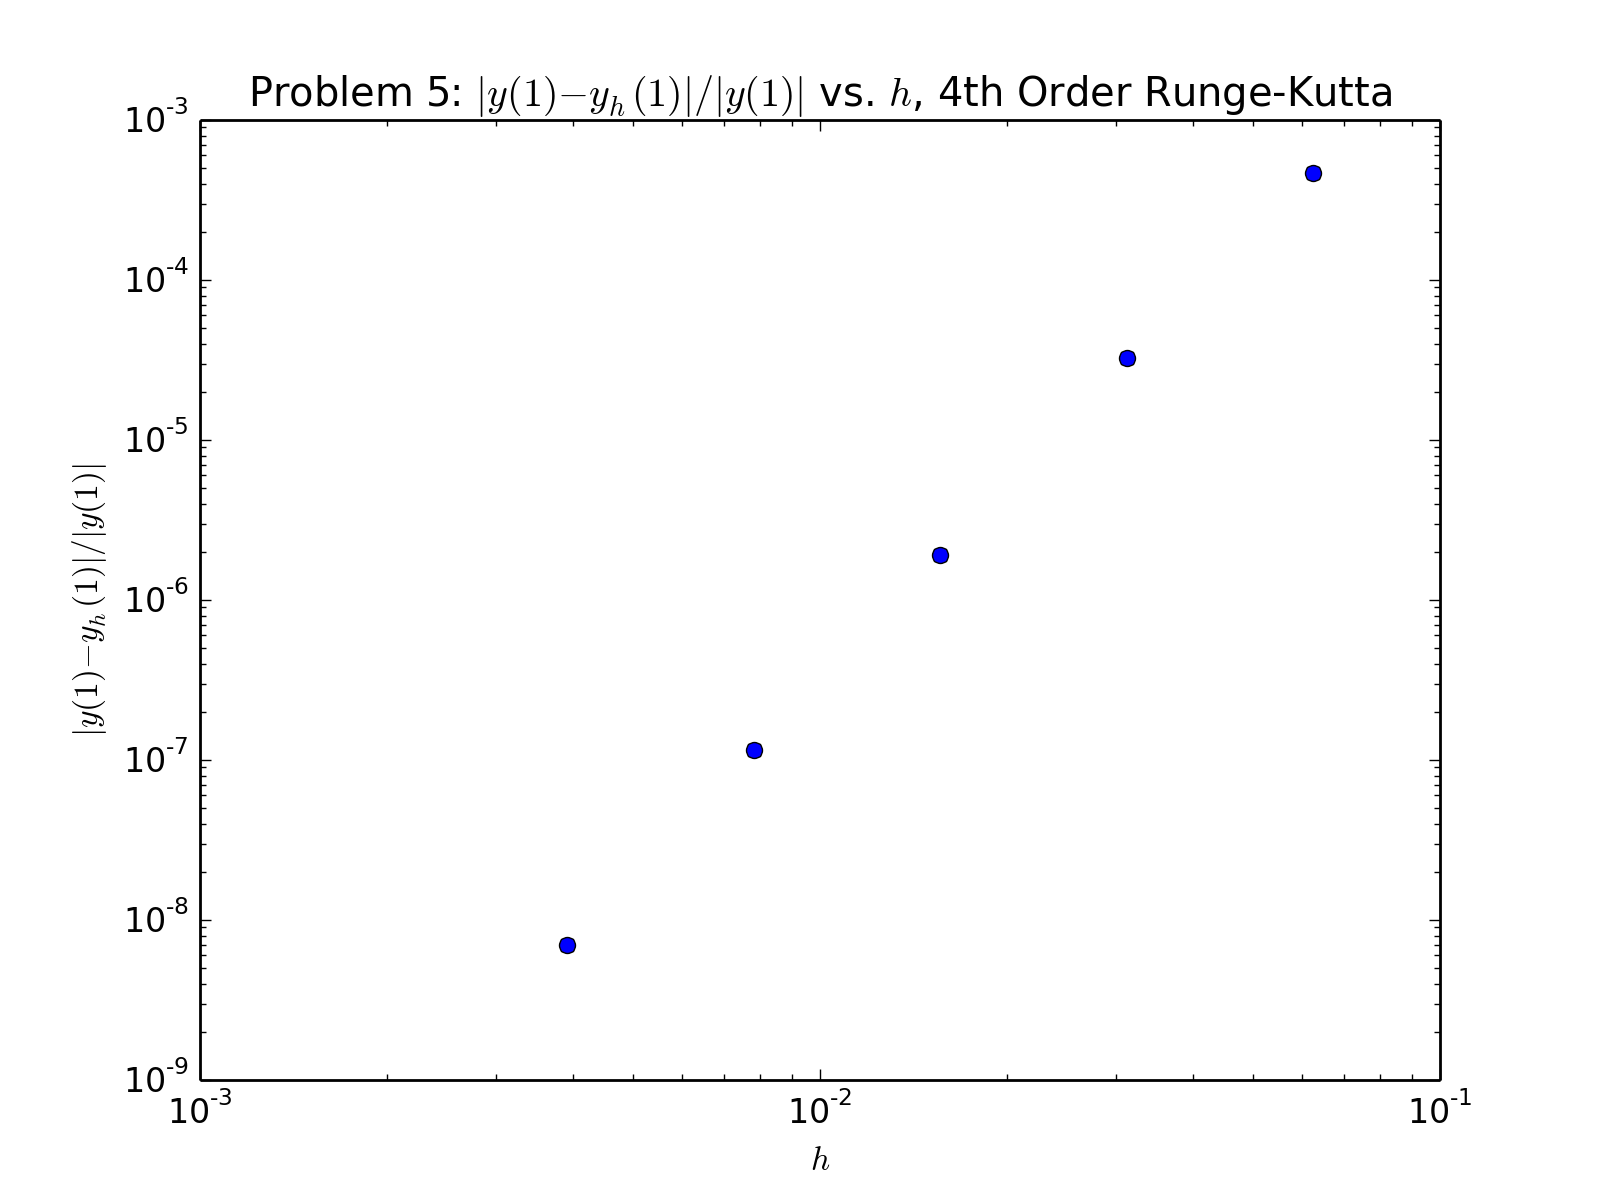
\includegraphics[scale=0.6]{ivp_err_rk}
\end{figure}

E.O.C. values: 3.83391337,  4.09025602,  4.06263359,  4.03447133.

Looks stable! As $h \to 0$, the approximate solutions are close to the true solution.

\end{itemize}

\end{document}
